\documentclass{jsarticle}
\usepackage{robomech}
\usepackage{graphicx}

\begin{document}
\makeatletter
\title{複数台の移動ロボットによる通行者情報地図の更新手法}
{}
{An Update Method of Human Frequency Map by Multiple Mobile Robots}
{}

\author{
\begin{tabular}{ll}
\hspace○学\hspace{1zw}横山光希 (明治大)& \hspace{1zw} 森岡一幸(明治大)\\
 &\\
 \multicolumn{2}{l}{\small Koki YOKOYAMA, Meiji University, y.koki0601@gmail.com}\\
 \multicolumn{2}{l}{\small Kazuyuki MORIOKA, Meiji University}
\end{tabular}
}
\makeatother

\abstract{ \small
By acquiring, sharing and updating sensor data in space on multiple robots and utilizing it with other robots, it is possible to efficiently recognize surrounding information and lead to better decision making.
In this research, we have developed a sensor data sharing system for mobile robot using block chain sharing Human Frequency Map as sensor data.
In this paper, we describe a method of updating multiple robot Human Frequency Map, and created a simulator and evaluated the method.
}

\date{} % 日付を出力しない
\keywords{Multiple robots, Human Frequency Map, Update Spatial Information}
\maketitle
\thispagestyle{empty}
\pagestyle{empty}

\small
\section{緒言}
自律移動ロボットは測域センサやカメラなどの情報に基づき周囲の環境を認識し行動をしている。
しかしロボット自身に搭載されているセンサデータだけでは取得できる情報に限界が存在する。
そこで空間に分散させたセンサノードから情報を取得する方法が提案されている。
これを空間の知能化という。
カメラを空間上に分散させロボットの人追従を行なった研究事例\cite{1}も報告されており、これによりロボットが外部のセンサ情報を利用する有用性が確認できる。
しかしこの手法ではセンサノードを空間内に設置する際に、設置位置などの詳細な設定を行う必要があるという問題点も存在する。

そこで本研究では環境にセンサノードを固定させるのではなく、同一空間上に存在する複数のロボットがセンサデータを取得・共有・更新を行う枠組みの提案および開発を目的としている。
著者らはセンサデータ共有の枠組みとしてブロックチェーンを用いたシステム提案し、開発に着手してきた\cite{2}。
またロボットが共有するセンサデータとして通行者情報地図(HFM:Human Frequency Map)を用いたシステムを提案し、開発を行なっている\cite{3}\cite{4}。
複数台の移動ロボットを同一空間上に存在させ、HFMを取得し共有するロボットと共有されたHFMを活用するロボットの開発を行なった。
しかしこのシステムではHFMを共有し、他のロボットが活用する流れの動作確認を目的としており、HFMを取得しにいく際には人間が手動でロボットを移動させていた。

本稿ではロボットが自動かつ継続的にHFMを更新しデータを蓄積する手法を提案する。
また本稿ではシミュレーターを作成し、提案手法の実験を行なった。


\section{提案システム}
本研究ではHFMを共有するセンサデータとしてシステムを提案し、その開発に着手してきた。
複数台の移動ロボットが地図空間の様々な場所に移動しHFMを観測する。
その観測したHFMをブロックチェーンを介し共有を行うことで、空間上にいる他のロボットもそのデータを活用するという一連の流れの開発を目的としている。
図\ref{fig: proposedsystem}は提案システムの全体像を示している。
この提案システムを実現するために次の4つの段階があると考える。
\begin{itemize}
  \item Acquire(HFMの取得)
  \item Share(HFMの共有)
  \item Utilize(HFMの活用)
  \item Update(HFMの更新)
\end{itemize}
著者らは取得・共有・活用までは\cite{4}で開発しているので、本稿ではHFMの更新を主な目的としている。


\begin{figure}[tbh]
 \centering
  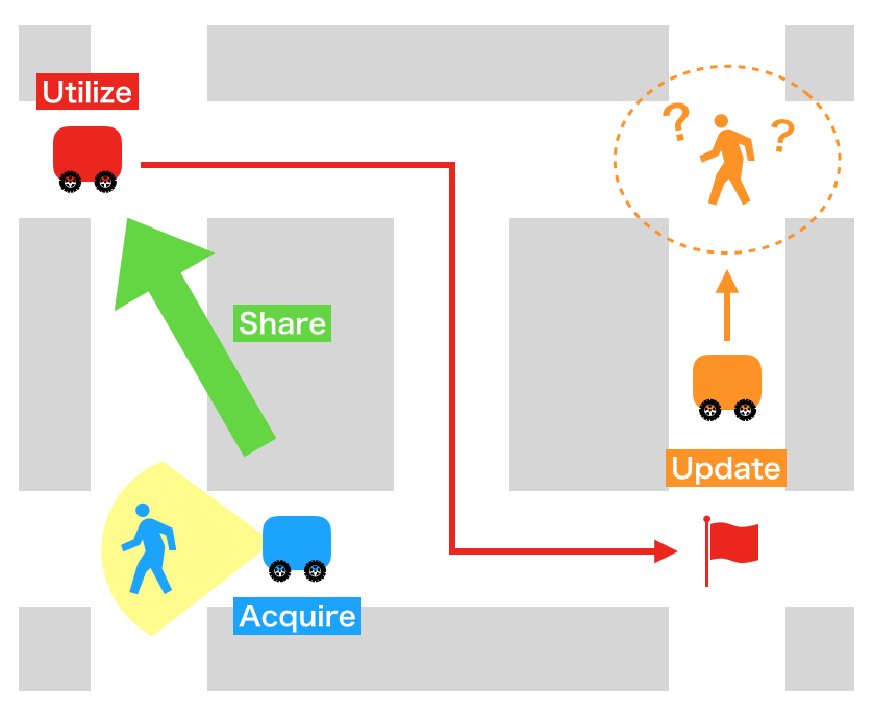
\includegraphics[height=50mm]{fig/proposedsystem.eps}
  \vspace*{-4mm}
  \caption{Proposed System}
  \label{fig: proposedsystem}
\end{figure}



\subsection{Human Frequency Map}
Human Frequency Mapとは占有格子地図をグリッドに分けた時にグリッドごと保持している人の経路情報のことである。
人の経路情報とは通行頻度や人の進行方向などのことである。
本研究では通行頻度を利用しており、図\ref{fig: HFM}はそのイメージを示している。
\begin{figure}[tbh]
 \centering
  \includegraphics[height=50mm]{fig/HFM.eps}
  \vspace*{-4mm}
  \caption{Human Frequency Map}
  \label{fig: HFM}
\end{figure}


\section{HFM更新手法}
\subsection{グリットごとの観測回数の共有}
HFMを更新していくためにはロボットが共有された情報を基に次の観測地点を決定していく必要がある。
そこでグリッドごとに観測回数を持たせ、それを共有すること手法をとる。
これを基にHFMを更新するロボットが次どこの地点を観測すればいいのかを判断する。
またこの手法ではHFMがブロックチェーン上で共有されるたびに観測されたグリッドの観測回数を更新する必要がある。
今回はHFMが共有されるのを監視するPCをブロックチェーンのノードして接続しこれを実現させる(図\ref{fig: sharefile})。

\begin{figure}[tbh]
 \centering
  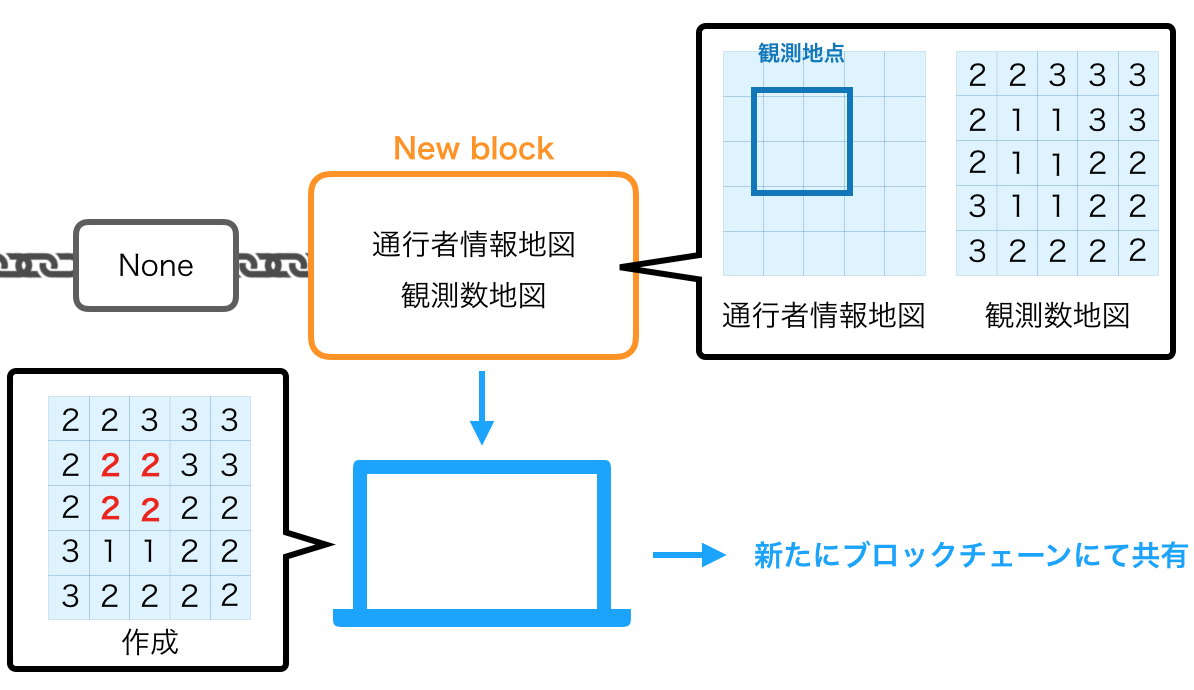
\includegraphics[height=40mm]{fig/sharefile.eps}
  \vspace*{-4mm}
  \caption{Share a Number of Observation}
  \label{fig: sharefile}
\end{figure}


\subsection{観測地点の決定方法}
\label{decide}
次の観測地点を決定する手段として、グリットごとの観測数とロボットの現時点からの距離を利用する。
本研究ではロボットを静止させ、前方6mx6mの範囲でHFMを観測を行わせているため、一度の観測における観測範囲は固定である。
その観測範囲に対応した矩形範囲内で地図の左上から右下まで探索を行い、
矩形範囲内ごとの平均観測数$x_{o}$およびロボットの現時点からの距離$x_{d}$を求める。
\reffig{fig: value-method}の青い矩形が矩形範囲内に相当し、矩形範囲内の左上のグリッドが距離である。
これらの数値にそれぞれ重み$w_{o},w_{d}$をかけ足し合わせたものを矩形範囲における$value$とする。

この$value$が最小の地点を次の観測地点と決定する。
\refeqn{eqn: value}は$value$の計算式である。

\begin{equation}
  value = w_{o}x_{o} + w_{d}x_{d}
	\label{eqn: value}
\end{equation}

$x_o,x_d$は絶対値の違いによる作用を考慮し、全ての矩形範囲での$x_o,x_d$を計算したのち、それぞれ標準化したものを利用している。
また$w_o,w_d$の範囲は0$\sim$1であり、\refeqn{eqn: weight}の条件を満たしている。

\begin{equation}
  w_o = 1 - w_d
	\label{eqn: weight}
\end{equation}


\begin{figure}[tbh]
 \centering
  \includegraphics[height=45mm]{fig/decisionpoint.eps}
  \vspace*{-4mm}
  \caption{Decision of Obsevation Point}
  \label{fig: value-method}
\end{figure}

\subsubsection{平均観測数の計算}
矩形範囲における平均観測数を変数として利用するためには矩形範囲内に存在する観測不可能なグリットの数を考慮する必要がある。
観測不可能なグリットとは壁や地図外の未確認の地点である。
そこで今回求める矩形範囲内の平均観測数は分母に矩形範囲内の観測可能なグリットの合計をとり、観測不可能グリットの影響を除去する。
\refeqn{eqn: distance}は矩形範囲内の平均観測数を求める式である。

\begin{equation}
  平均観測数 = \frac{観測回数の合計}{観測可能なグリット数}
	\label{eqn: observation}
\end{equation}

\subsubsection{距離の計算}
距離の計算においてはグリット単位での計算を行なっている。
本研究でも一辺0.5mのグリットを利用している。
\refeqn{eqn: distance}は距離の計算式である。
ここでは$ロボットの現時点での座標を(x_0, y_0)、次の地点を(x_1,y_1)$とし表している。


\begin{equation}
  distance = \sqrt{(x_0-x_1)^2 + (y_0-y_1)^2}
	\label{eqn: distance}
\end{equation}



\section{シミュレーターの開発}
\label{simulation}
本稿では実際にロボットに走行させるではなく、シミュレーターを開発し観測回数の遷移および最適な重みの探索を行う。今回のシミュレーターはpythonにて開発を行なった。
\subsection{シミュレーション手順}
\label{process-simulation}
\begin{enumerate}
  \item グリットごとの観測数の初期化(全て0にする)
  \item ロボットの初期位置を決定(地図上の地点からランダムに決定)
  \item \ref{decide}項の手法により観測地点の決定
  \item 決定した観測地点をもとにグリットごとの観測数を+1
\end{enumerate}
手順の3,4を任意の回数繰り返すことにより、地図全体の観測回数の遷移を確認することができる。
この任意の回数のことをここでは試行回数$n$と呼ぶこととする。
また$w_o,w_d$はプログラム上で変更することができる。
図\ref{fig: example of simulation}は初期段階から試行回数を1度行なった時の図である。
上の画像が観測数が初期の図であり、赤く囲まれた部分が初期地点として観測を行った地点であり、観測数が増えているのがわかる。

\begin{figure}[tbh]
 \centering
  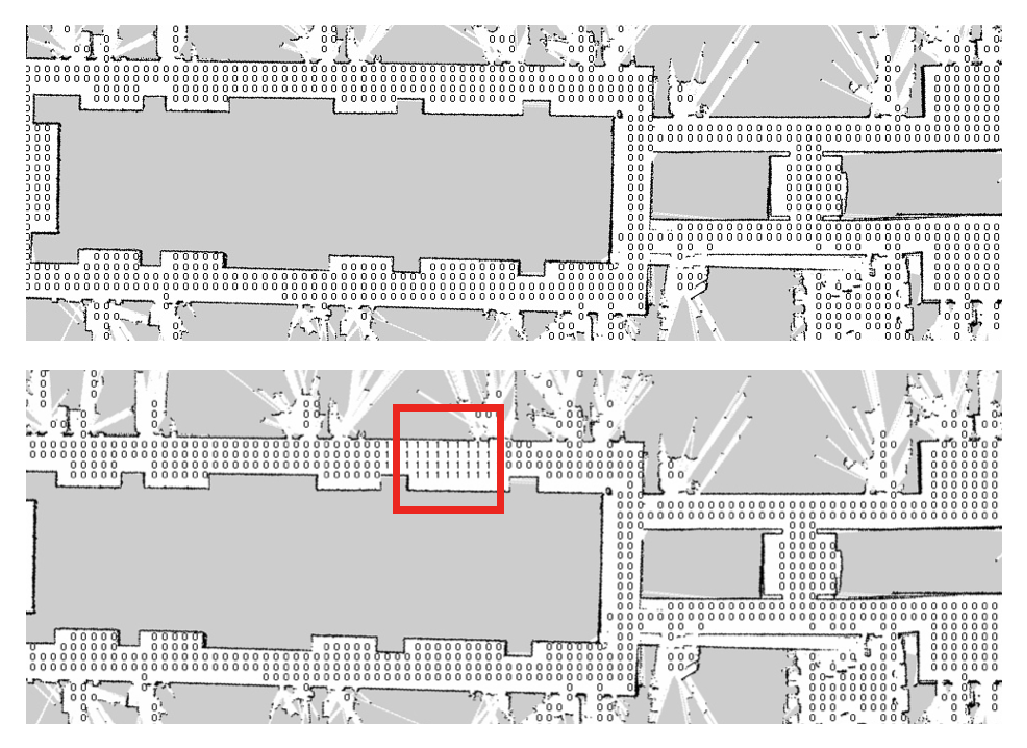
\includegraphics[height=55mm]{fig/example.eps}
  \vspace*{-4mm}
  \caption{Example of Simulation}
  \label{fig: example of simulation}
\end{figure}

\subsection{シミュレーション実験}
\label{run-simulation}
\ref{process-simulation}項で開発したものを明治大学中野キャンパス11Fの地図にてシミュレーションを行う。
$n=1000,w_o=1.0,w_d=0.0$とし、シミュレーションを行なった。
これは距離を無視することにより、観測回数のみを考慮した数値を得ることができると考えたためである。
図\ref{fig: result of experiments}のグラフはその結果である。
横軸が試行回数$n$、縦軸が地図全体の平均観測数である。
地図全体の平均観測数は以下の\refeqn{eqn: average-in-map}で定義している。
また地図全体で観測可能なグリット数はこの地図では1272箇所である。

\begin{equation}
  地図全体の平均観測数 = \frac{地図全体の観測回数の合計}{地図全体の観測可能なグリット数}
	\label{eqn: average-in-map}
\end{equation}

\begin{figure}[tbh]
 \centering
  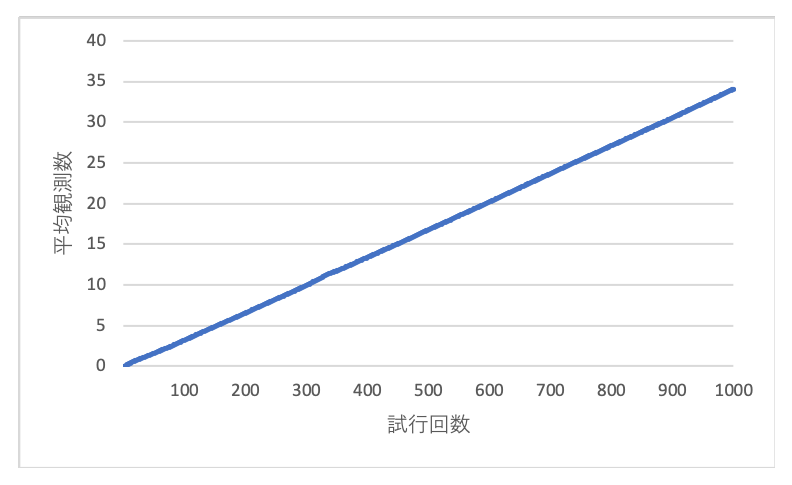
\includegraphics[height=40mm]{fig/n1000.eps}
  \vspace*{-4mm}
  \caption{Result of Experiment}
  \label{fig: result of experiments}
\end{figure}

この結果より距離を考慮しない場合、試行回数$n=1000$の時地図全体の平均観測数が約35回になることがわかる。
つまりこの実験環境においておおよそ試行回数$n=30$で全てのグリットの観測を行うことができる。
図\ref{fig: n30}は試行回数$n=30$の時のグリットごとの観測数を地図に描画したものであり、ほとんどのグリットにおいて観測数が1か2なのがわかる。


\begin{figure}[tbh]
 \centering
  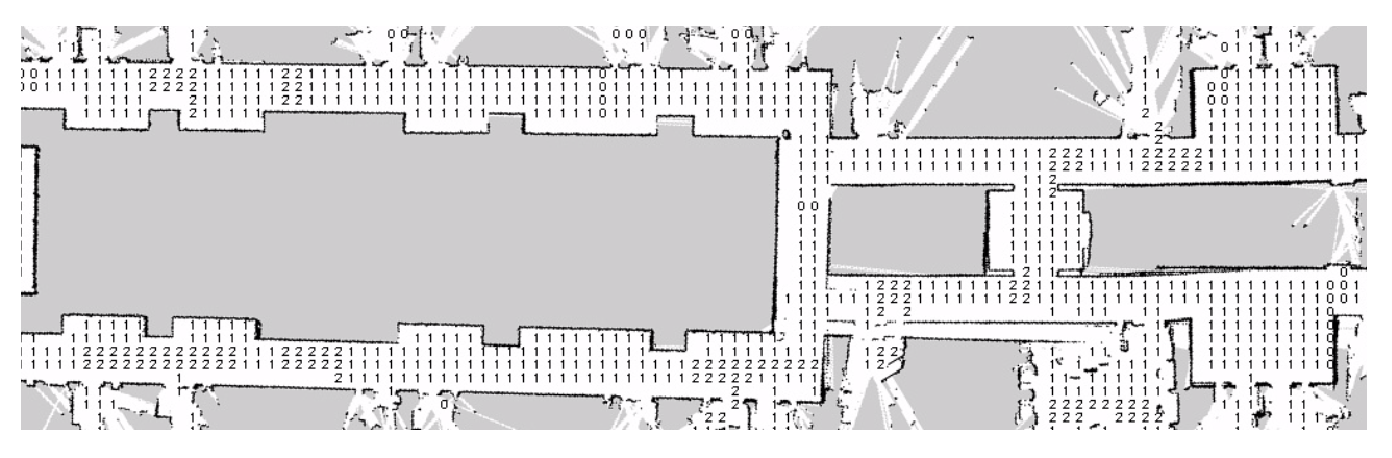
\includegraphics[height=25mm]{fig/n30.eps}
  \vspace*{-4mm}
  \caption{試行回数$n=30$}
  \label{fig: n30}
\end{figure}




\section{重みの評価}
\ref{simulation}章で開発したシミュレーターを用いて最適な$w_o,w_d$の探索を行う。
本稿では以下の2点に着目し重みの評価を行った。
\begin{itemize}
	\item 観測したグリッド数の比較
	\item 総距離の比較
\end{itemize}
\ref{run-simulation}項により試行回数が約30で全てのグリッドを観測するのわかった。
そこでシミュレーション上にて距離の重みを0$\sim$1の範囲で0.1ずつ変化させ、
それぞれの重みで30回の試行回数を5回行うことにする。
5回シミュレーションを行ったあと結果の平均を取り、それぞれの重みでの比較を行う。


\subsection{観測したグリッド数の比較}
\label{evaluate-observation}
地図全体で観測可能なグリットは1272箇所あり、試行回数30の際に1272箇所に近いグリット数を観測するのが理想的である。
そこで$w_d$で観測グリット数を算出し比較を行う。
図\ref{fig: evaluate-observation}は$w_d$ごとの観測したグリット数のグラフである。


\begin{figure}[tbh]
 \centering
  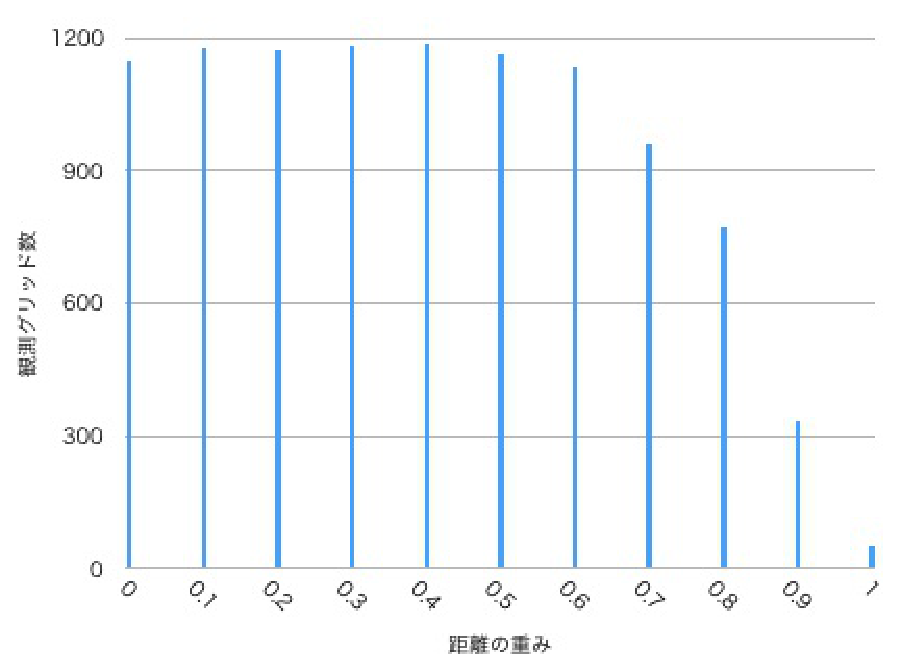
\includegraphics[height=50mm]{fig/evaluate-grid.eps}
  \vspace*{-4mm}
  \caption{観測したグリット数による評価}
  \label{fig: evaluate-observation}
\end{figure}


\subsection{総距離の比較}
\label{evaluate-distance}
地図全体の観測を効率的に行うためには、距離を最小限に行なっていく必要がある。
図\ref{fig: evaluate-distance}は$w_d$ごとの総距離のグラフである。


\begin{figure}[tbh]
 \centering
  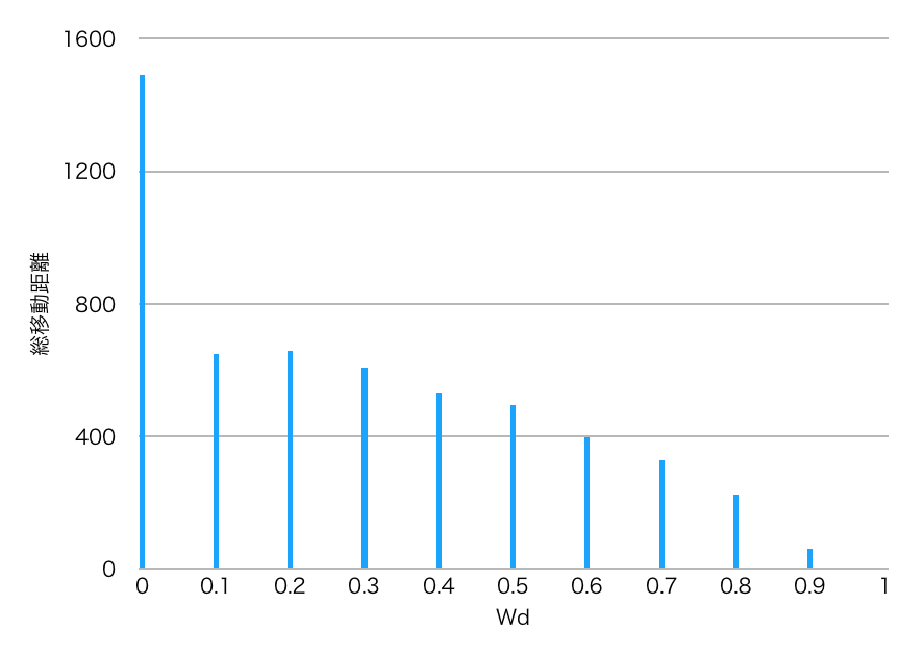
\includegraphics[height=50mm]{fig/evaluate-distance.eps}
  \vspace*{-4mm}
  \caption{総距離による評価}
  \label{fig: evaluate-distance}
\end{figure}

\subsection{重みの評価に対する考察}
図\ref{fig: evaluate-observation}から$w_d$が0.5までは観測回数が1200弱で横並びであり、それ以降減少していることがわかる。
また図\ref{fig: evaluate-distance}から$w_d$が増えるにあたり、総距離が少なくなっていることがわかる。
この結果から$w_d$は0.5前後が最適だと考えられる。

\section{複数台のロボットを想定したシミュレーション}
\subsection{シミュレーション内容および結果}

前章までに行なったシミュレーションはロボットが1台として実験を行なっている。
そこでロボットの数を増やした時の場合を想定した時のシミュレーションを行う。
観測したグリット数が試行を繰り返すごとにどのように遷移していくかをロボットの数ごとに比較を行う。
今回ロボットの数は1$\sim$3台,試行回数$n=30,w_o=0.5,w_d=0.5$とし、シミュレーションを行なった。
ロボットの台数によりシミュレーションを5回ずつ行い、その結果をそれぞれ平均をとったものを図\ref{fig: multirobot}のグラフにて示す。
ロボットの台数によりシミュレーションを5回ずつ行い、その結果をそれぞれ平均したものを利用し台数ごとの比較を行う。
図\ref{fig: each-multirobot}が台数ごとの結果、図\ref{fig: multirobot}が平均を取り比較した結果のグラフである。
ともに横軸は試行回数$n$,縦軸は観測したグリット数となっている。

\begin{figure}[tbh]
 \centering
  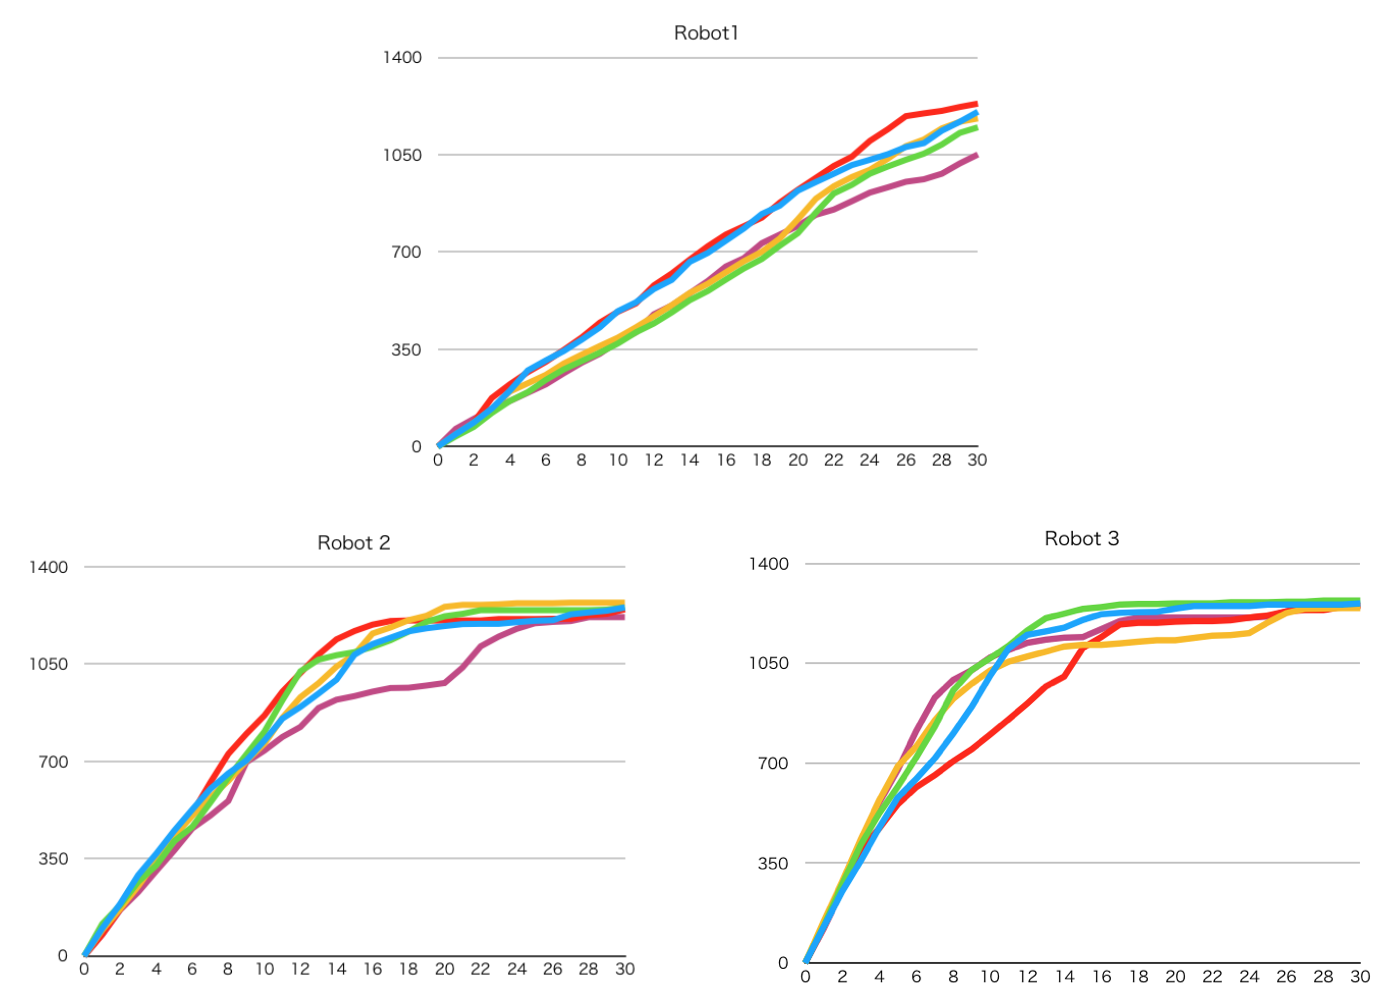
\includegraphics[height=55mm]{fig/each-multi-robot.eps}
  \vspace*{-4mm}
  \caption{それぞれの台数での結果}
  \label{fig: each-multirobot}
\end{figure}

\begin{figure}[tbh]
 \centering
  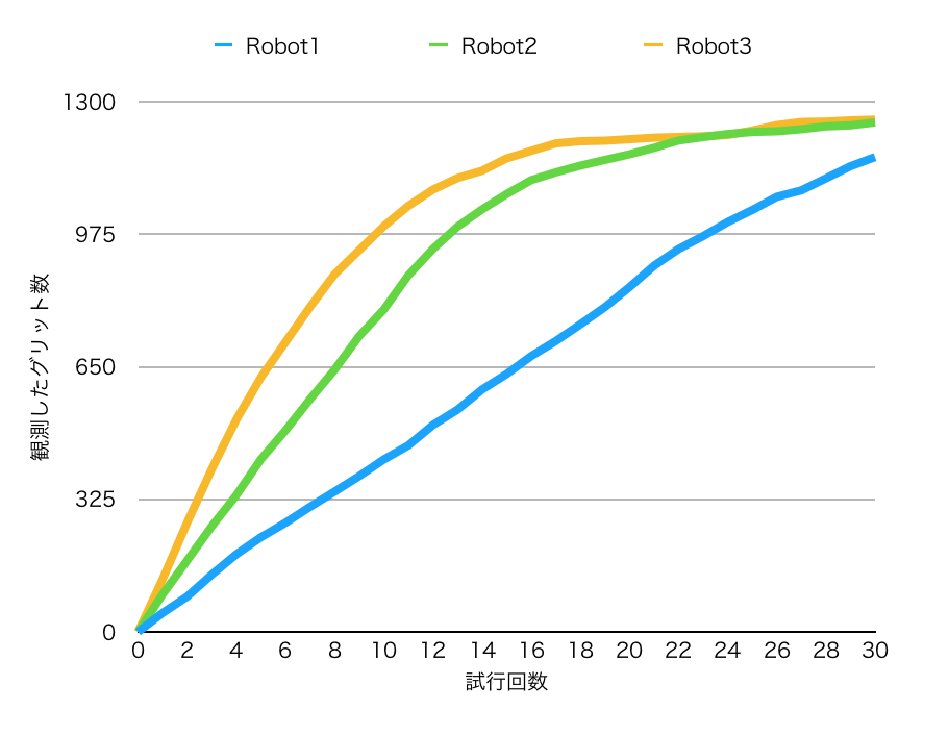
\includegraphics[height=50mm]{fig/multi-robot.eps}
  \vspace*{-4mm}
  \caption{複数台ロボット}
  \label{fig: multirobot}
\end{figure}


\subsection{シミュレーションに対する考察}
図\ref{fig: multirobot}からロボットの数が増えるほど少ない試行回数で地図全体のグリットを観測できることがわかる。
これより今回提案した手法を用い複数台のロボットで観測を行うことで、効率的に地図全体のHFMの観測を行うこができることを確認することができた。




\section{結言}
本稿では通行者情報地図を共有情報とし、それを更新していくための手法について提案した。
またシミュレーションを開発し、その手法に対する検証も行なった。
しかし今回の手法およびシミュレーション以下のことが考慮されていない。
\begin{itemize}
  \item 今回の距離は単なる点と点との距離でしかなく、実際のロボットの移動距離でなはい。
  \item 観測地点でのロボットの位置、向きという情報は設定されていない。
  \item 矩形範囲内は全て+1しているので、壁などの影響で同時に観測できない地点もカウントしてしまっている。(図\ref{fig: impossible})
\end{itemize}
\begin{figure}[tbh]
 \centering
  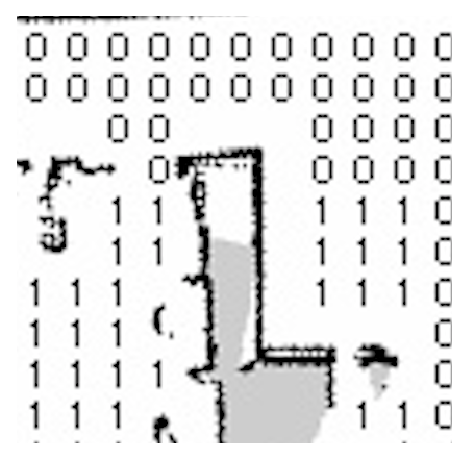
\includegraphics[height=30mm]{fig/impossible.eps}
  \vspace*{-4mm}
  \caption{同時に観測不可な地点}
  \label{fig: impossible}
\end{figure}

今後は上記を考慮したシミュレーターを作成し提案手法の評価を行い、実環境での実験を目指す。


\footnotesize
\begin{thebibliography}{99}

\bibitem{1}
Kazuyuki Morioka, Joo-Ho Lee, Hideki Hashimoto, "Human- following mobile robot in a distributed intelligent sensor network", IEEE Transactions on Industrial Electronics, Vol.51, No.1, pp.229-237, 2004.

\bibitem{2}
横山光希, 森岡一幸, "ブロックチェーンを用いた知能化空間のためのセンサデータ共有システム", ROBOMECH2018. 2A2-D08, 2018.

\bibitem{3}
横山光希, 森岡一幸, "ブロックチェーンを用いた移動ロボットのための環境地図共有システム", SI2018. 2D4-06, 2018.

\bibitem{4}
加藤勇気, 森岡一幸, “移動ロボットによる人間観測に基づく通行者情報の作成と柔軟な経路計画”, ROBOMECH2017, 2A2-D08, 2017.




\end{thebibliography}

\normalsize
\end{document}
